% Author: Seongjin Lee
% Hanyang University, Seoul, Korea
% esos.hanyang.ac.kr
% 2016-09-20
% note: some slides are adopted from  \url{www.cs.stevens.edu/~jschauma/631A/}
% https://github.com/resourceful/lecture_sysprog/

\documentclass[newPxFont,sthlmFooter,nooffset]{beamer}
\usepackage{kotex}
%\usetheme{sthlm}
\usepackage{../beamer_template/beamerthemesthlm}
\hypersetup{pdfauthor={Seongjin Lee (insight@gnu.ac.kr)},
            pdfsubject={Lecture Note: System Programming},
            pdfkeywords={Lecture Note, System Programming, class, (under)graduate},
            pdfmoddate={D: \pdfdate},
            pdfcreator={Seongjin Lee}}

%\setbeamertemplate{footline}[text line]{%
%    \parbox{\linewidth}{\vspace*{-8pt} \insertsectionhead  \hfill\insertshortauthor\hfill\insertpagenumber}}
%\setbeamertemplate{navigation symbols}{}




\title{System Programming}
\subtitle{Chapter 7: Process Environment}
\author{Atieh Sahraei}
\institute{Systems Research Lab.\\Gyeongsang National University}
\date{\today}

\begin{document}



\frame[plain]{\titlepage}

\frame{\frametitle{Table of contents}\tableofcontents}


%---------------------------------------------------------




\section{Process Environment}

\begin{frame}[t]
  \frametitle{Introduction}
In this chapter, we'll see
\begin{itemize}
\item how the \texttt{main} function is called when the program is executed
\item how command-line arguments are passed to the new program
\item what the typical memory layout looks like
\item how to allocate additional memory
\item how the process can use environment variables
\item and various ways for the process to terminate
\item the \texttt{longjmp} and \texttt{setjmp} functions and their interaction with the stack
\end{itemize}

\end{frame}



\subsection{Process Creation and Termination }

\begin{frame}[containsverbatim,t]
  \frametitle{\texttt{main} Function}
\begin{codedef}
int main(int argc, char *argv[]);
\end{codedef}
\begin{itemize}
\item \textit{argc}: the number of commands-line arguments
\item \textit{argv}: an array of pointers to the arguments
\end{itemize}

When a C program is executed by one of exec functions, a special start-up routine is called before the main function is called;
\begin{itemize}
\item This start-up routine takes values from the kernel---the
  command-line arguments and the environment---and sets things up
\end{itemize}

\end{frame}



\begin{frame}[t]
  \frametitle{Process Termination}

There are eight ways for a process to terminate

Normal termination
\begin{itemize}
\item Return from \texttt{main}
\item Calling \texttt{exit}
\item Calling \texttt{\_exit} or \texttt{\_Exit}
\item Return of the last thread from its start routine
\item Calling \texttt{pthread\_exit} from the last thread
\end{itemize}

Abnormal termination (Details in next chapters)
\begin{itemize}
\item calling \texttt{abort}
\item Receipt of a signal
\item Response of the last thread to a cancellation request
\end{itemize}

\end{frame}

\begin{frame}[containsverbatim,t]
  \frametitle{exit(3) Functions}
Following functions terminate a program normally
\begin{codedef}
#include <stdlib.h>
void exit(int status); // return to the kernel after some cleanup
void _Exit(int status); // return to the kernel immediately

#include <unistd.h>
void _exit(int status);  // return to the kernel immediately
\end{codedef}

\end{frame}

\begin{frame}[t]
  \frametitle{exit(3) Functions}
All three exit functions expect a single integer argument, which we
call the exit status. E.g., \texttt{exit(0);}

Most UNIX System shells provide a way to examine the exit status of a
process.

The exit status of the process is undefined, if
\begin{itemize}
\item any of these functions is called without an exit status,
\item main does a return without a return value, or
\item the main function is not declared to return an integer,
\end{itemize}

Returning an integer value from the main function is equivalent to calling exit with the same value. Thus

\texttt{exit(0);}
is the same as
\texttt{return(0);}
\end{frame}


\begin{frame}[containsverbatim,t]
  \frametitle{exit(3) function example}
\bigskip
  \begin{columns}
    \begin{column}{0.45\linewidth}
      The classic ``hello, world'' example
      \lstinputlisting[linerange={13,18},lineskip=-5pt]{codes/hello.c}
    \end{column}
    \begin{column}{0.5\linewidth}
\begin{verbatim}
$ make hello
$ ./hello
hello, world
^C
$ echo $?
130
\end{verbatim}
\texttt{\$?} prints exit status of previous process

      more on exit status
      \url{http://tldp.org/LDP/abs/html/exitcodes.html}
    \end{column}
  \end{columns}
\end{frame}

\begin{frame}[containsverbatim,t]
  \frametitle{atexit(3) function}
With ISO C, a process can register at least 32 functions that are automatically called by
\texttt{exit}. These are called \textit{exit handlers} and are registered by calling the \texttt{atexit} function.

\begin{codedef}
#include <stdlib.h>
int atexit(void (*func)(void));
// Returns: 0 if OK, nonzero on error
\end{codedef}


\end{frame}


\begin{frame}[t]
  \frametitle{How Process are Created and Terminated}

\begin{figure}[h]
  \centering
  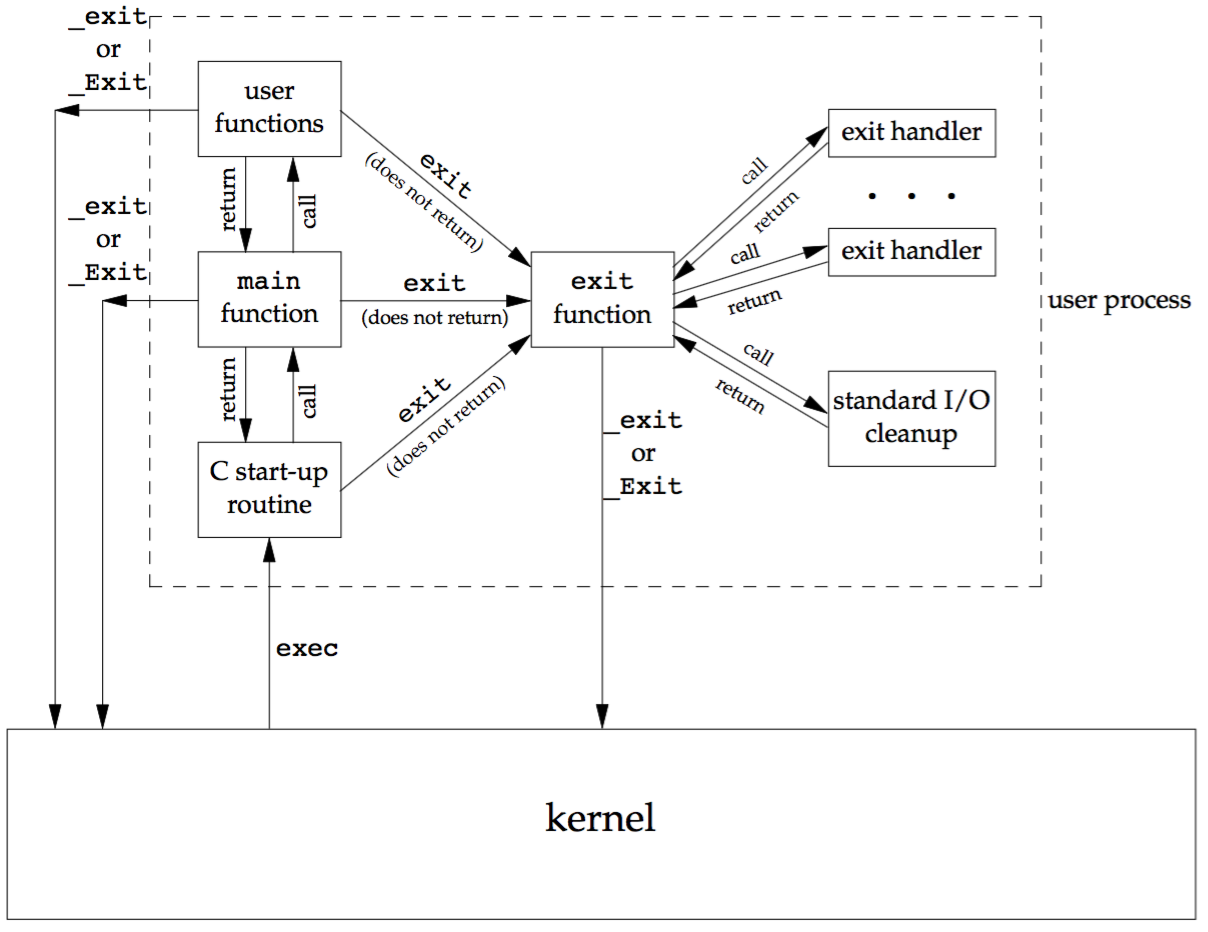
\includegraphics[height=0.85\textheight]{figure/fig7-2_how_prog.png}
  \caption{How a C program is started and how it terminates}
\end{figure}
\end{frame}





\subsection{Environments}

\begin{frame}
  \frametitle{Command-Line Arguments}
When a program is executed, the process that does the exec can pass command-line arguments to the new program.

\texttt{cd codes; make echoall}

\lstinputlisting[lineskip=-5pt]{codes/echoall.c}

try,
\texttt{./echoall arguments tests}

If compile this program
\begin{itemize}
\item \texttt{argv[0]: ./echoall}
\item \texttt{argv[1]: arguments}
\item \texttt{argv[2]: tests}
\end{itemize}
\end{frame}

\begin{frame}[t]
  \frametitle{Environment List}
Each program is also passed an environment list
\begin{itemize}
\item it is an array of character pointers
\item each pointer containing the address of a null-terminated C
  string
\item The address of the array of pointers is contained in the global variable environ \texttt{extern char **environ;}
\end{itemize}

\begin{figure}[h]
  \centering
  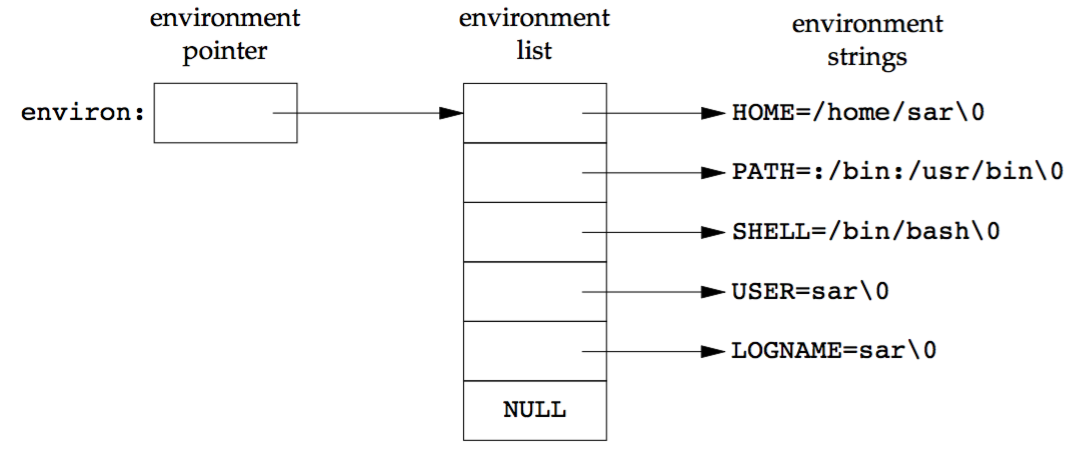
\includegraphics[width=0.7\textwidth]{figure/fig7-5_environment.png}
  \caption{Environment consisting of five C character strings}
\end{figure}
\end{frame}

\begin{frame}[t]
  \frametitle{Environment Variables}
\begin{figure}[h]
  \centering
  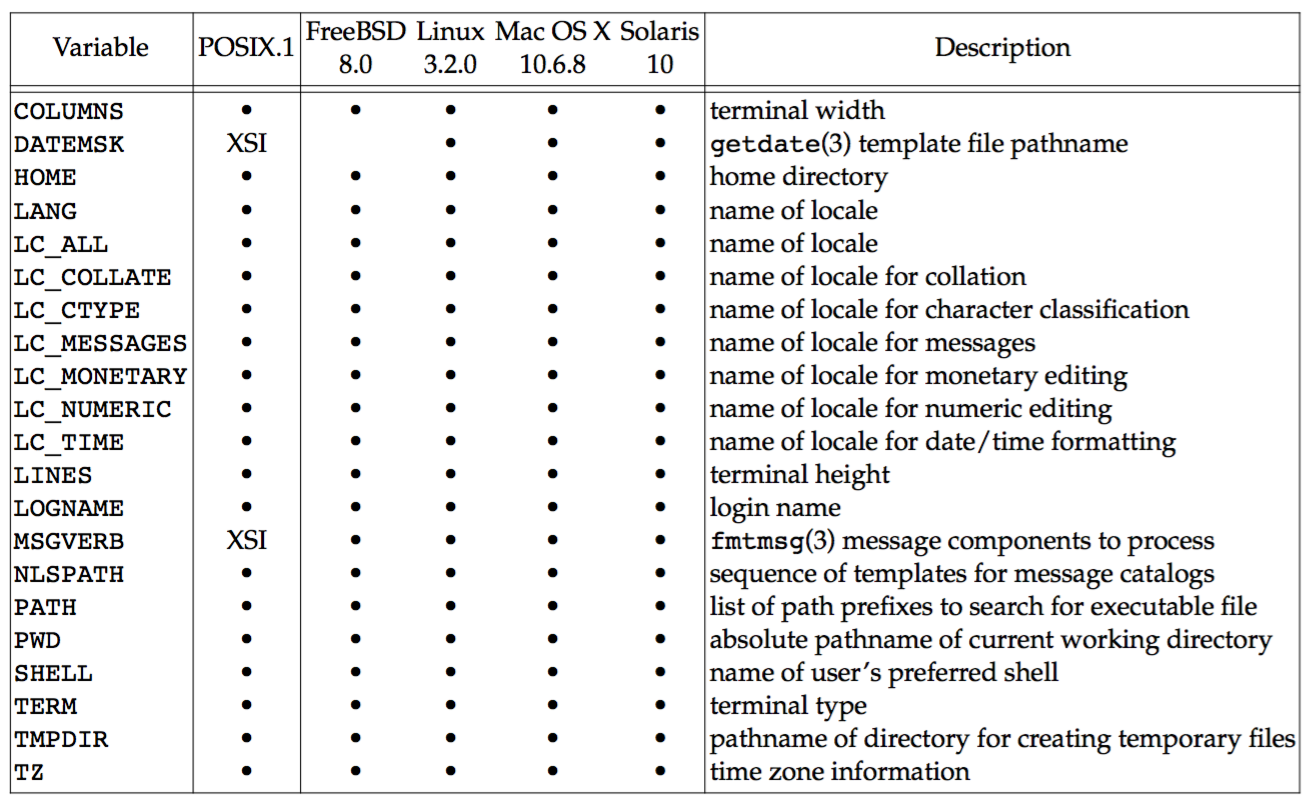
\includegraphics[width=0.9\textwidth]{figure/fig7-7_environment.png}
  \caption{Environment consisting of five C character strings}
\end{figure}
\end{frame}

\begin{frame}[t]
  \frametitle{Environment List cnt'd}
ISO C specifies that the main function be written with two arguments

POSIX.1 specifies that environ should be used instead of the (possible) third argument
\begin{itemize}
\item Access to specific environment variables is normally through the
  \texttt{getenv} and \texttt{putenv} functions
\item But to go through the entire environment, the environ pointer must be used
\end{itemize}

\end{frame}



\begin{frame}[containsverbatim,t]
  \frametitle{Environment List APIs}

\begin{codedef}
#include <stdlib.h>
char *getenv(const char *name);
// Returns: pointer to value associated with name, NULL if not found
int putenv(char *str);
// Returns: 0 if OK, nonzero on error
int setenv(const char *name, const char *value, int rewrite);
int unsetenv(const char *name);
// Both return: 0 if OK, −1 on error
\end{codedef}
{\footnotesize
\begin{table}[h]
  \centering
  \begin{tabular}{l | c c | *{4}{c}  }
    Fuction & ISO C & POSIX.1 & \parbox{5em}{\centering FreeBSD 8.0} & \parbox{5ex}{\centering Linux 3.2.0} & \parbox{5em}{\centering Mac OS X 10.6.8} & \parbox{5em}{\centering Solaris 10} \\ \hline \hline
    getenv  & $\bullet$ & $\bullet$ & $\bullet$ & $\bullet$ & $\bullet$ & $\bullet$ \\
    putenv  &           &   XSI     & $\bullet$ & $\bullet$ & $\bullet$ & $\bullet$ \\
    setenv  &           & $\bullet$ & $\bullet$ & $\bullet$ & $\bullet$ &           \\
  unsetenv  &           & $\bullet$ & $\bullet$ & $\bullet$ & $\bullet$ &           \\
  clearenv  &           &           &           & $\bullet$ &           &           \\
  \end{tabular}
  \caption{Support for various environment list functions}
  \label{tab:support}
\end{table}
}
\end{frame}


\subsection{Memory}


\begin{frame}[t]
  \frametitle{The Pieces of a C program}
  \begin{description}
  \item[Text segment] Machine instructions for CPU. It is sharable. It is \textbf{read-only} to prevent from accidental modification
  \item[Initialized data segment] Or, data segment. Contains variables that are specifically initialized in the program \\
\texttt{int maxcount = 99;}
\item[Uninitialized data segment] Often called the ``bss'' segment (A.K.A ``block started by symbol'') \\
\texttt{long sum[1000];}
\item[Stack] Automatic variables are stored. Each time a function is called, the address of where to return to and info about the caller's environment (i.e., registers) are saved on the stack.
\item[Heap] dynamic memory allocation.
  \end{description}


\end{frame}




\begin{frame}
  \frametitle{Memory Layout of a C Program}
  \begin{figure}[h]
    \centering
    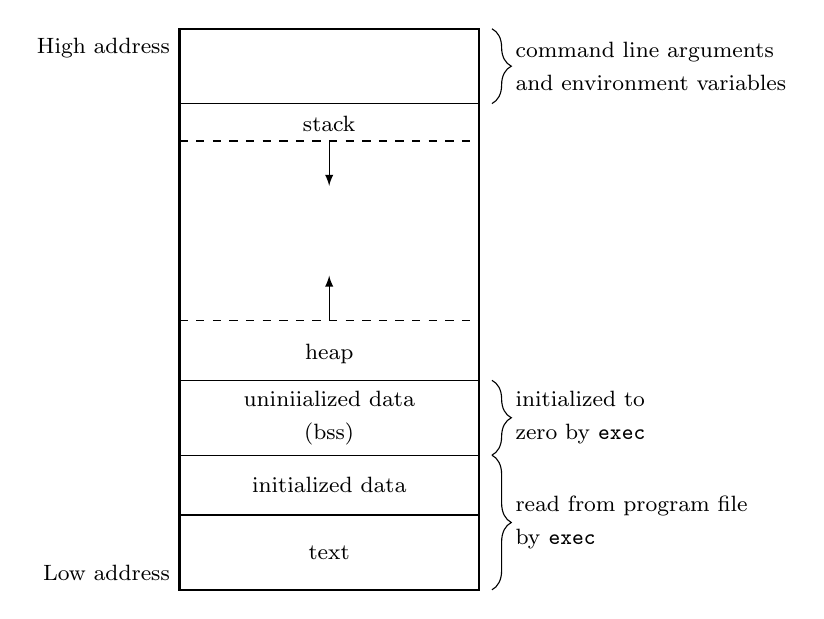
\begin{tikzpicture}[scale=0.95]
      % the box
      \draw [black, thick] (0,0) rectangle (4,7.5);
      \node [align=right, above left] at (0, 0) {\footnotesize Low address};
      \node [align=right, below left] at (0, 7.5) {\footnotesize High address};

      % high address before stack
      \uncover<2->{ \draw [black, thin] (0,6.5) -- (4,6.5);}
      % brace
      \uncover<2->{ \draw [decorate,decoration={brace,amplitude=7pt},xshift=5pt,yshift=0pt] (4,7.5) -- (4,6.5) node [black,align=left,midway,right, xshift=5pt] {\footnotesize command line arguments \\ \footnotesize and environment variables}; }

      % text
      \uncover<3->{ \draw [black, thin] (0,0) rectangle (4,1) node [black, align=center, midway] {\footnotesize text};}
      % initialized data
      \uncover<4->{ \draw [black, thin] (0,1) rectangle (4,1.8) node [black, align=center, midway] {\footnotesize initialized data};}
      % brace
      \uncover<4->{ \draw [decorate,decoration={brace,amplitude=7pt},xshift=5pt,yshift=0pt] (4,1.8) -- (4,0) node [black,align=left,midway,right, xshift=5pt] {\footnotesize read from program file \\ \footnotesize by \texttt{exec}};}
      % uninitialized data
      \uncover<5->{ \draw [black, thin] (0,1.8) rectangle (4,2.8) node [black, align=center, midway] {\footnotesize uniniialized data \\ \footnotesize (bss)};}
      % brace
      \uncover<5->{ \draw [decorate,decoration={brace,amplitude=7pt},xshift=5pt,yshift=0pt] (4,2.8) -- (4,1.8) node [black,align=left,midway,right, xshift=5pt] {\footnotesize initialized to \\ \footnotesize zero by \texttt{exec}};}

      % stack
      \uncover<6->{ \draw [dashed, thin] (0, 6) -- (4,6) node [black, align=center, midway, above] {\footnotesize stack};}
      % arrow down
      \uncover<6->{ \draw [arrows=-latex] (2,6) -- (2, 5.4);}

      % heap
      \uncover<7->{ \draw [dashed, thin] (0, 3.6) -- (4,3.6) node [black, align=center, midway, below, yshift=-5pt] {\footnotesize heap};}
      % arrow up
      \uncover<7->{ \draw [arrows=-latex] (2,3.6) -- (2, 4.2);}
    \end{tikzpicture}\\[1em]
    \caption{Typical Memory arrangement}
\label{fig:memory}
\end{figure}

\end{frame}

\begin{frame}[containsverbatim,t]
  \frametitle{Shared Libraries}
\texttt{size(1)} command reports the size (in bytes) of the text, data, and bss segments.

Compare the size of a program before and after static linking.
\bigskip
{\footnotesize

    Static linking:
\begin{verbatim}
gcc -static -o hello hello.c
$ls -l hello
-rwxr-xr-x 1 atieh  879443 Oct 30 10:39 hello
$size hello
text    data    bss    dec     hex  filename
787775    6128  11272  805175  c4937  hello
\end{verbatim}
    Dynamic linking:
\begin{verbatim}
$ gcc -o hello hello.c
$ls -l hello
-rwxr-xr-x 1 atieh  8378 Oct 30 10:39 hello
$size hello
  text    data    bss    dec     hex  filename
  1176     504     16   1696     6a0  hello
\end{verbatim}

}
\end{frame}

\begin{frame}[containsverbatim,t]
  \frametitle{Advantages of Shared Libraries}
\begin{itemize}
\item Remove common library routines from executable file
\item Maintain a single copy of library routine in memory
\item Reduces the size of executable file
\item Library functions can be replaced with new versions without having to edit every program that uses the libarary.
\end{itemize}
\end{frame}

\begin{frame}[containsverbatim,t]
  \frametitle{Memory Allocation}

\begin{codedef}
#include <stdlib.h>
void *malloc(size_t size);
void *calloc(size_t nobj, size_t size);
void *realloc(void *ptr, size_t newsize);
// All three return: non-null pointer if OK, NULL on error

void free(void *ptr);
\end{codedef}
\begin{description}
\item[\texttt{malloc}] allocates a specified number of bytes of memory. The initial value of the memory is indeterminate
\item[\texttt{calloc}] allocates a specified number of bytes of memory and initializes them to 0 bits
\item[\texttt{realloc}] increases or decreases the size of a preivously allocated area
\item[\texttt{free}] deallocates the area. Do not \texttt{free} what is already freed
\end{description}

\end{frame}

\begin{frame}[containsverbatim,t]
  \frametitle{Errors Causes by Memory Allocation}
\begin{itemize}
\item Writing past the end or before the start of an area could overwrite the record block.
\item Freeing a block that was already freed.
\item Calling free with a pointer that was not obtained from one of the alloc functions.
\item Forget to call free after calling malloc, cause memory leakage.
\end{itemize}
\end{frame}

\subsection{Misc.}

\begin{frame}[containsverbatim,t]
  \frametitle{\texttt{setjmp} and \texttt{longjmp} Functions}
In C, we can't \texttt{goto} a label that's in another function. Instead, we must use the \texttt{setjmp} and \texttt{longjmp} functions to perform this type of branching
\begin{codedef}
 #include <setjmp.h>
int setjmp(jmp_buf env);
// Returns: 0 if called directly, nonzero if returning from a call to longjmp
void longjmp(jmp_buf env, int val);
\end{codedef}
\begin{itemize}
\item call \texttt{setjmp} from the location that we want to return to.
  \begin{itemize}
  \item \texttt{jmp\_buf} data type is some form of array that is capable of holding all the information required to restore the status of the stack to the state when we call \texttt{longjmp}
  \end{itemize}
\item when we encounter an error, we call \texttt{longjmp} with two arguments
  \begin{itemize}
  \item \texttt{jmp\_buf env} used in \texttt{setjmp}
  \item \texttt{val} is nonzero value that becomes the return value from \texttt{setjmp}
  \end{itemize}
\end{itemize}
\end{frame}

\begin{frame}[containsverbatim,t]
  \frametitle{\texttt{setjmp} and \texttt{longjmp} interactions with stack}\lstinputlisting[lineskip=-5pt]{codes/skel_cmd.c}

\end{frame}

\begin{frame}[containsverbatim,t]
  \frametitle{\texttt{setjmp} and \texttt{longjmp} interactions with stack Cnt'd}

\begin{figure}[h]
  \centering
  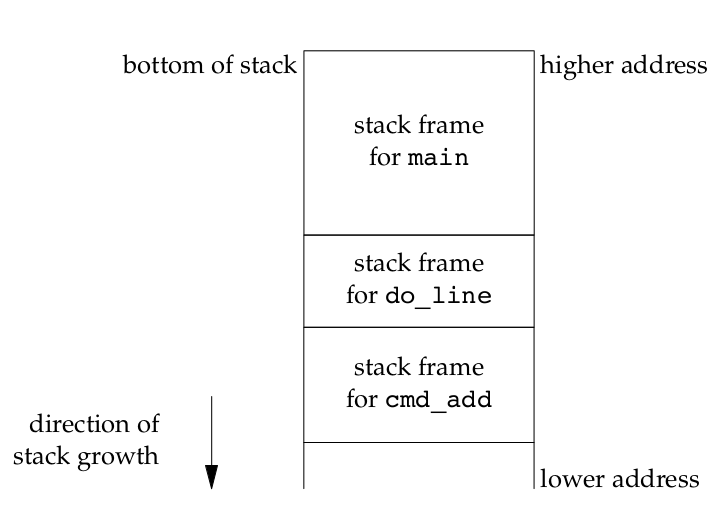
\includegraphics[width=0.7\textwidth]{figure/fig7-10_environment.png}
  \caption{Stack frames after \texttt{cmd} has been called}
\end{figure}

\end{frame}

\begin{frame}[containsverbatim,t]
  \frametitle{\texttt{setjmp} and \texttt{longjmp} interactions with stack Cnt'd}

\lstinputlisting[lineskip=-5pt]{codes/jmp.c}

\end{frame}

\begin{frame}[containsverbatim,t]
  \frametitle{\texttt{setjmp} and \texttt{longjmp} interactions with stack Cnt'd}

\begin{figure}[h]
  \centering
  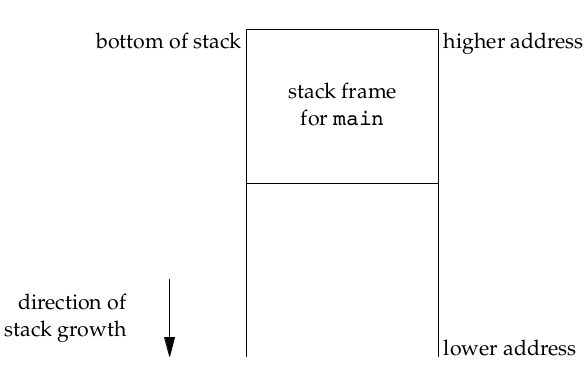
\includegraphics[width=0.7\textwidth]{figure/fig7-12_environment.png}
  \caption{Stack frames after \texttt{longjmp} has been called}
\end{figure}

\end{frame}

\end{document}
